\section{Supplementary Material}
\beginsupplement

\section{Full confounder test}
\label{sup:full-test}

The full confoudner test generates a null-distribution for an arbitrary predefined test statistic $T(\y,\yhat,\c)$ by sampling permutation based "copies" of $\y$,

$$\y_i^{(j)} \sim Q(\cdot|c_i) \ $$

where, $Q(.|c)$ denotes the conditional distribution of $\y$ given $\c=c$ and $j=1,\dots, m$ indexes the "copy" of $\y$ so that $\y^{(i)} = (y_1^{(j)}, \dots, y_n^{(j)})$ is a permutation of the original vector $\y = (y_1, \dots, y_n)$. This mechanism creates copies $\y^{(1)}, \dots ,\y^{(m)}$ that are exchangeable with the original vector $\y$ under the null hypothesis that $\yhat \independent \y | \c$.

Under the null hypothesis, the triples $$(\y,\yhat,\c), (\y^{(1)}, \yhat, \c),\dots, (\y^{(1)}, \yhat, \c)$$ are all identically distributed and exchangeable, and so are the 
$$T(\y,\yhat,\c), T(\y^{(1)}, \yhat, \c),\dots,T(\y^{(m)}, \yhat, \c)$$
test statistics, as well.

The p-value under the null hypothesis is then obtained as
$$ p= \frac{\sum_{j=1}^m \mathbb{1} \{T(\y^{(j)}, \yhat, \c) \geq T(\y, \yhat, \c) \}  }{m}$$

Let $S_n$ denote the set of all permutations on the indices $\{1,\dots,n\}$ and $\y_\pi = (y_{\pi_1}, \dots, y_{\pi_n})$ the vector $\y$ with its elements reordered according to the permutation $\pi \in S_i$.
The permutation-based copies of $\y$ are then of $\y^{(j)} = \y_{\pi^{(j)}}$ which are drawn so that:

\begin{equation}
    \mathbb{P}(\pi^{(j)} = \pi | \y,\yhat,\c) = \frac{q^n(\y_\pi | \c)}{\sum_{\pi' \in S_n} q^n(\y_{\pi'} | \c)}
    \label{eq-pperm}
\end{equation}

that is, according to the $q^n(\cdot|\c) := q(\cdot | c_1) \dots q(\cdot|c_n)$ product density corresponding to the conditional distribution $Q(\cdot|\c)$. Note that Eq. \ref{eq-pperm} does not necessarily assume a continuous distribution.
For a verification of the valid type I error control of this approach refer to Theorem 1 in \citep{berrett2020conditional}.

\begin{figure}[H]
  \centering
  \fbox{
   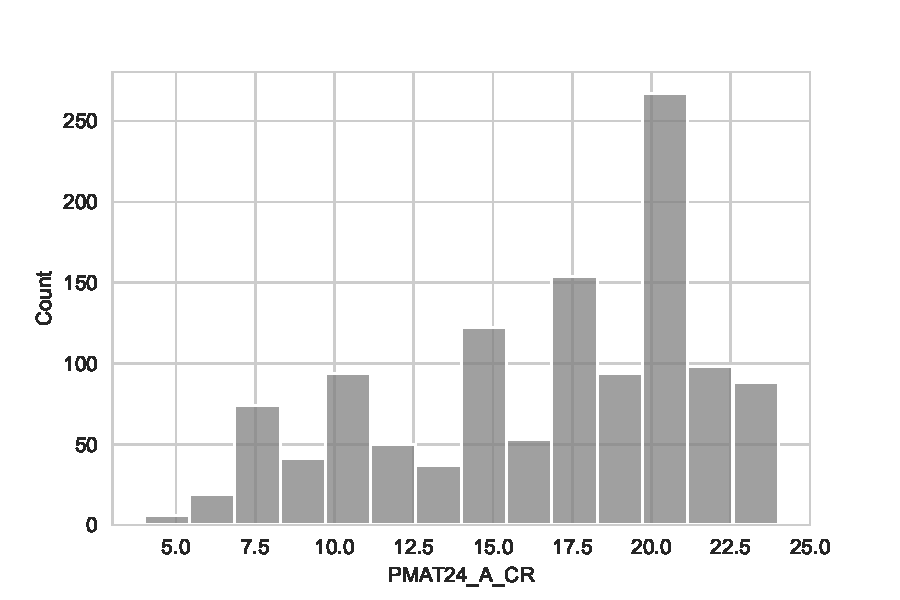
\includegraphics[width=0.36\paperwidth]{fig/supplement/hcp_iq_nonnorm_hist.pdf}
   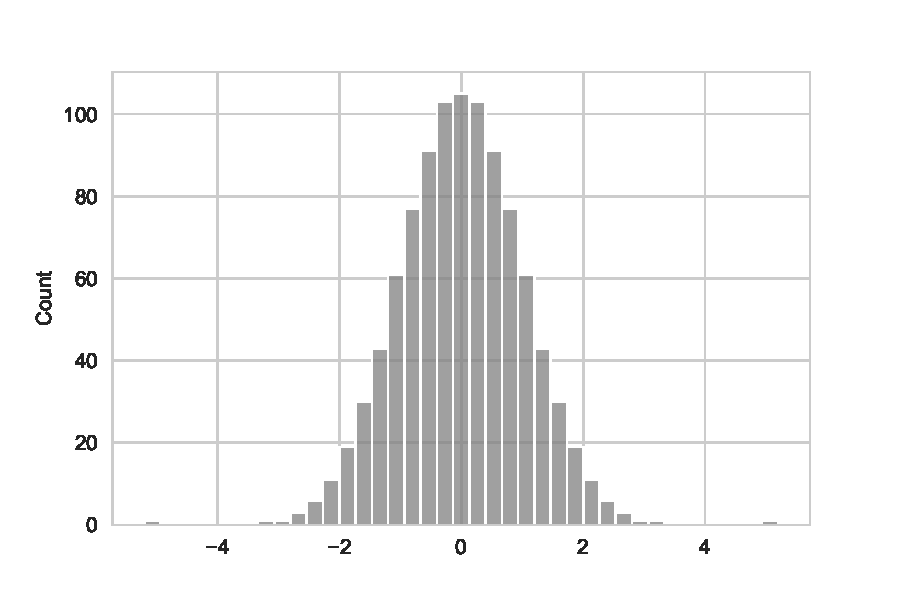
\includegraphics[width=0.36\paperwidth]{fig/supplement/hcp_iq_quanttrf_hist.pdf}
   }
  \caption{Histogram of fluid intelligence score in the HPC dataset, before (left) and after (right) quantile transformation.}
  \label{fig:hcp-hist}
\end{figure}

\begin{figure}[H]
  \centering
  \fbox{
   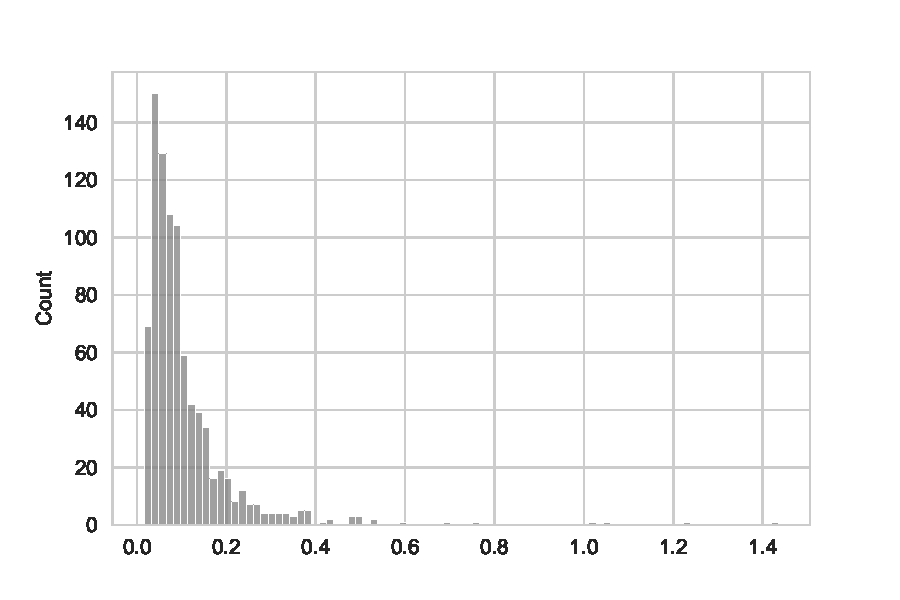
\includegraphics[width=0.36\paperwidth]{fig/supplement/abide_motion_hist.pdf}
   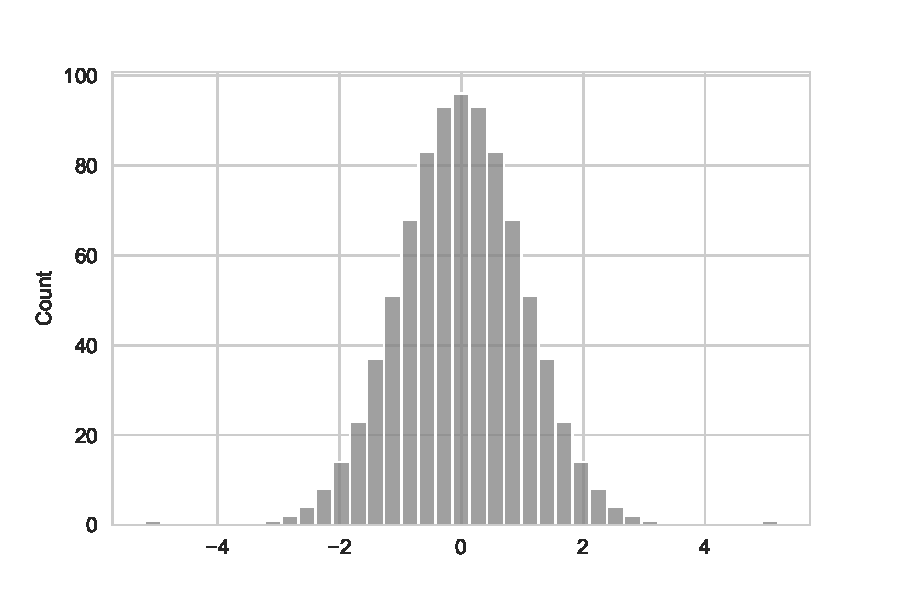
\includegraphics[width=0.36\paperwidth]{fig/supplement/abide_motion_quanttrf_hist.pdf}
   }
  \caption{Histogram of mean framewise displacement in the ABIDE dataset, before (left) and after (right) quantile transformation.}
  \label{fig:abide-hist}
\end{figure}

\begin{figure}[H]
  \centering
  \fbox{
   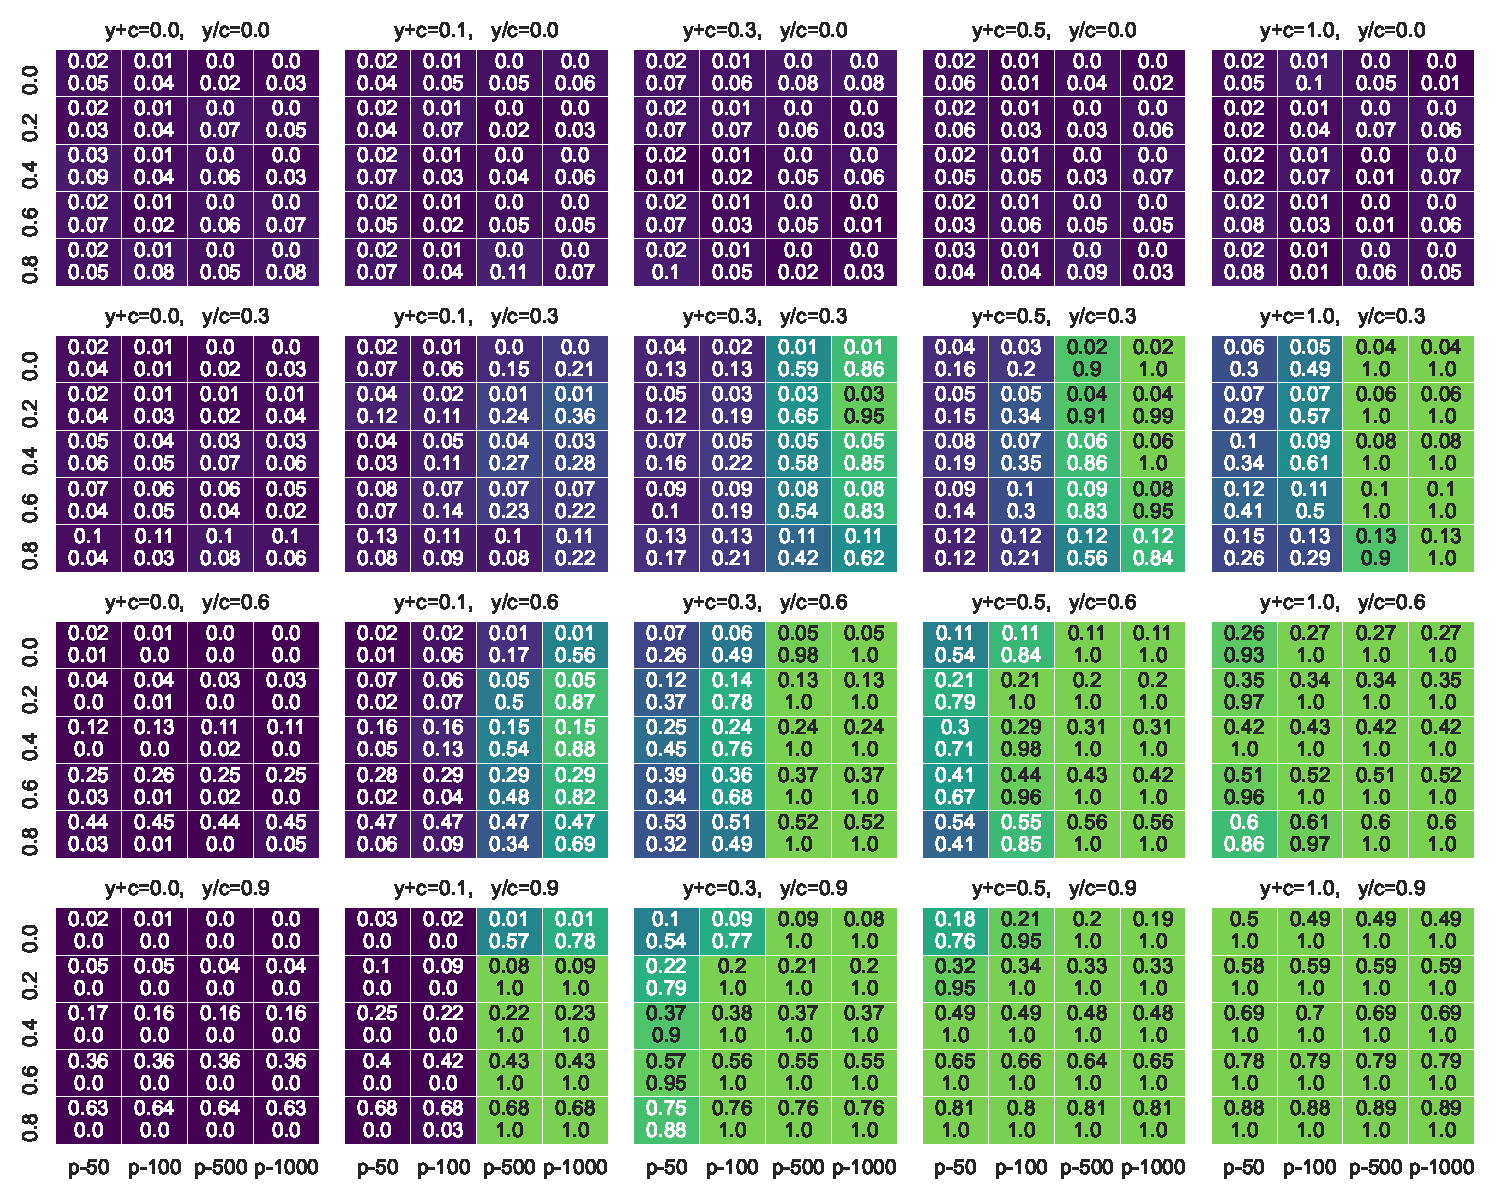
\includegraphics[width=0.75\paperwidth]{fig/supplement/sim_ccc_full_normal_all_heatmap.pdf}}
  \caption{Heatmaps showing the positive rates of the 'full' confounder test, with normally distributed numerical simulated variables.}
  \label{fig:sim-ccc-full}
\end{figure}


\begin{figure}[H]
  \centering
  \fbox{
   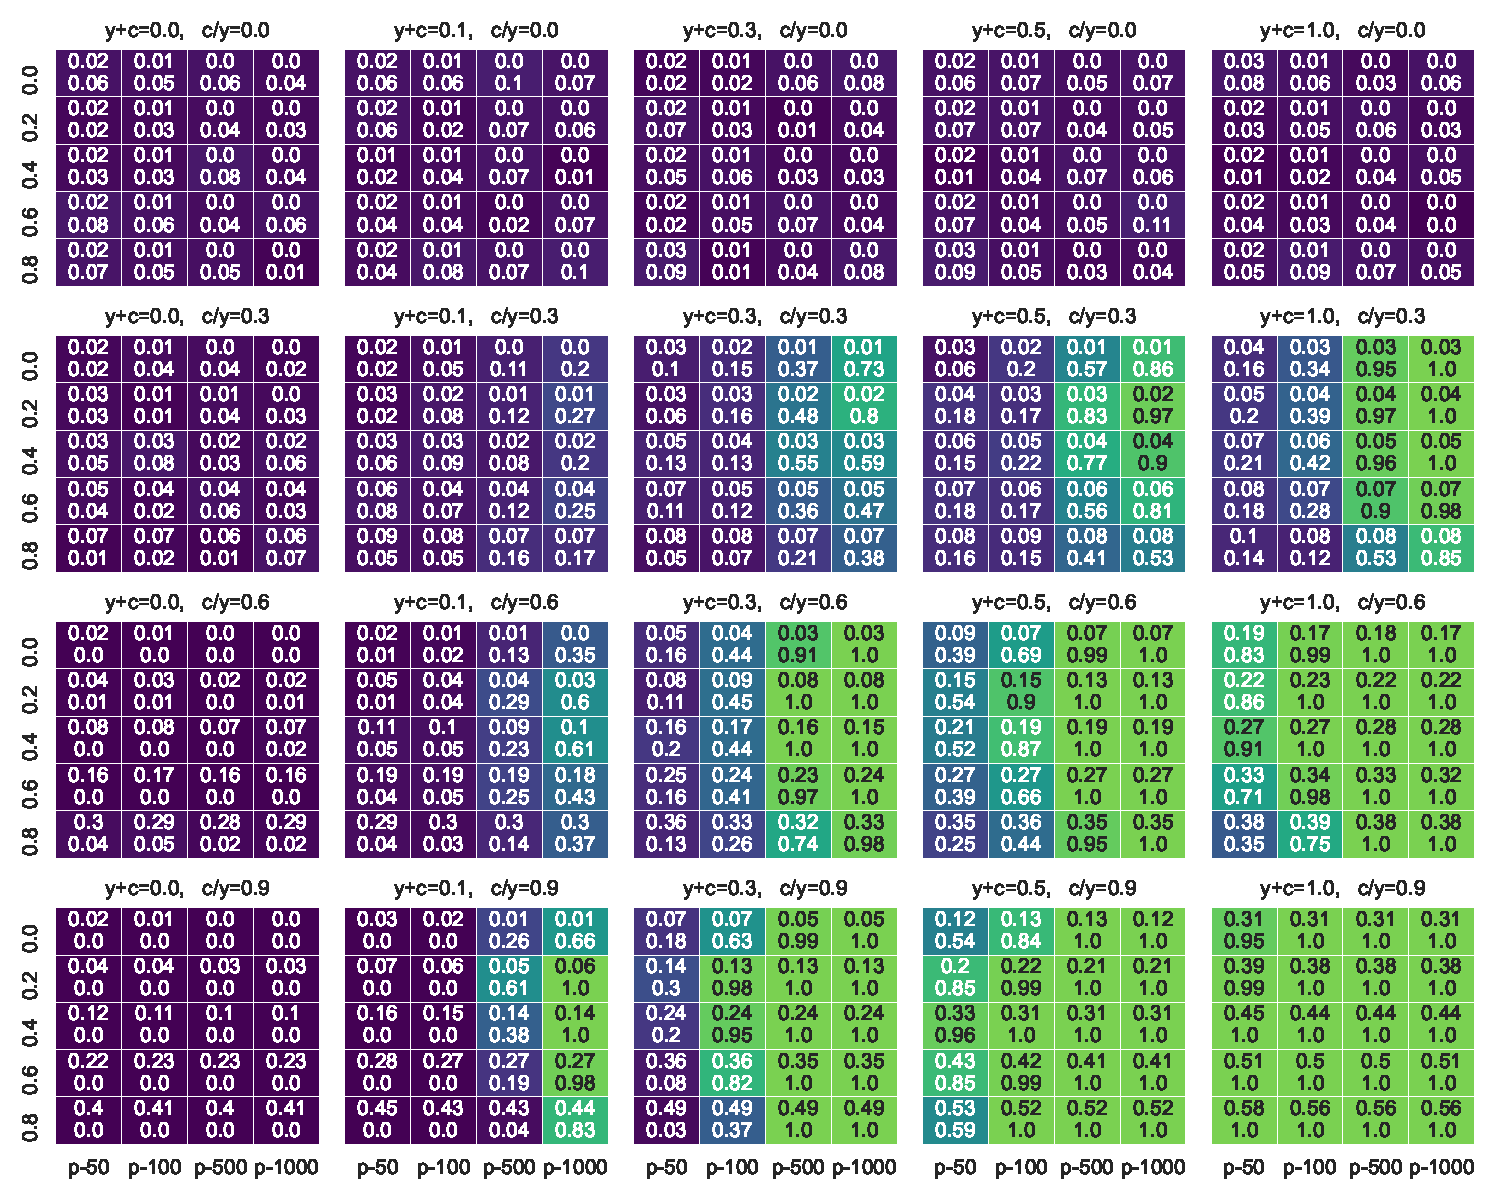
\includegraphics[width=0.75\paperwidth]{fig/supplement/sim_ccb_partial_normal_all_heatmap.pdf}}
  \caption{Heatmaps showing the positive rates of the 'partial' confounder test, with normally distributed numeric $Y$ and $\hat{Y}$ and categorical $C$.}
  \label{fig:sim-ccb-partial}
\end{figure}